\section{Appendix}

The PEC activity was studied in 3.5\% w/v NaCl in DI water. Linear sweep voltammetry (LSV) was performed directly on as-synthesized samples with chopped illumination at 1.5 sun in both sweep directions, with visible bubbles appearing upon the electrode surface when illuminated at potentials >1.18 V vs RHE (Figure \ref{fig:HeterostructuresCyclicVoltammetry} a, b, Figure S8). An early onset of measureable photocurrent at +0.48 V vs RHE was observed with the maximum on off ratio at +1.01 V vs RHE (Figure S8 a). A bare gold foil, which had been subjected to the CVD process without the addition of Mo, W, or S precursors, was used as a control and showed no catalytic activity for water oxidation. 

%\begin{figure}[h]
%	\begin{center}
%		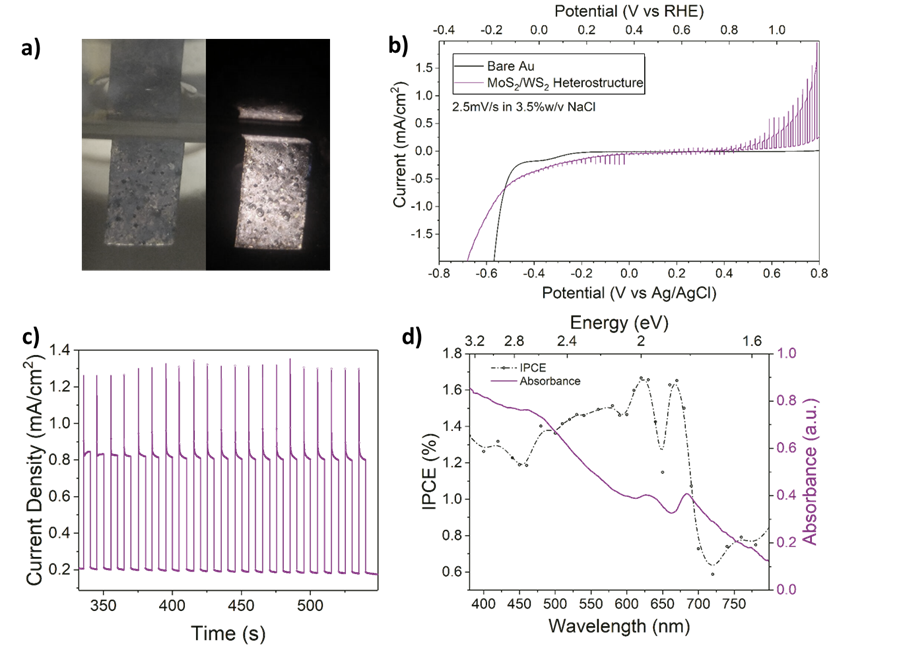
\includegraphics[scale=0.3]{Heterostructures/CyclicVoltammetry.png}
%		\caption{Photoelectrochemical characterisation of MoS2/WS2 heterostructure on gold in 3.5\% w/v NaCl in DI water; (a) Photograph of active electrode at +0.75 V vs Ag/AgCl, left: no-illumination, right: illuminated, showing gas bubble formation; (b) linear sweep voltammetry at 2.5 mV/s from +0.8 to -0.8 V vs Ag/AgCl demonstrating the complete protection of the Au surface as minimal noble-metal hydrogen evolution is observed and negligible contribution of the substrate to either dark or photocurrent in the water oxidation region; (c) chronoamperometry at +0.75 V vs Ag/AgCl with chopped illumination at 0.2 Hz; and (d) photocurrent dependence on monochromatic light at +0.75 V vs Ag/AgCl and corresponding absorbance spectra of the heterostructures dispersed via sonication in ethanol.}
%		\label{fig:HeterostructuresCyclicVoltammetry}
%	\end{center}
%\end{figure}

At potentials below +0.4 V vs RHE an inversion of the photocurrent was observed with significant instantaneous charge generation, however, negligible stable photocurrent was generated (Figure \ref{fig:HeterostructuresCyclicVoltammetry} b). This contribution arises due to the ambipolar characteristics of the TMDCs. In order to probe this effect, two stage chronoamperometry (CA) at -0.6 V vs Ag/AgCl and +0.75 V vs Ag/AgCl with chopped illumination was performed (Figure S8 b). The result of the chopped illumination at negative potentials was a slow increase in negative current flow upon illumination, which was recovered at approximately the same rate when the light source was blocked. When switched to positive potentials the previously described rapid water oxidation photocurrent was observed. 
CA performed at +1.129 V vs RHE, chosen to avoid oxygen bubble formation on the electrode surface, presented rapid charge generation immediately upon illumination followed by a stable photocurrent of 0.62 mA/cm2 at 1.5 sun illumination intensity (Figure \ref{fig:HeterostructuresCyclicVoltammetry} c) (0.4 mA/$cm^2$ at 1 sun, Figure S8 e). Sharp slopes in the chronoamperometry profiles collected  under chopped illumination were observed, suggesting a faster charge carrier recombination as compared to liquid phase processed material \cite{Pesci2017}. The observed fast kinetics of charge carrier recombination allowed for photocurrent to be obtained at frequencies up to 1 Hz, while a stable photocurrent under constant illumination was observed for over 10 minutes (Figure S8 e).  The photocurrent was confirmed to arise from the generation of oxygen through the use of an oxygen selective electrode, with an increase in the dissolved O2 concentration from 5 to 17 $\mu$mol/L upon illumination for 300 s (Figure S9). The Faradaic Efficiency (FE) for O2 generation was calculated to be 83 ± 15\%, indicating a high proportion of photogenerated holes being available to produce oxygen. The use of monochromatic light to obtain incident-photon-to-current efficiency (IPCE) demonstrates that the photocurrent mimics the reflectance spectra of the heterostructure, with IPCE of ~1.7\% at 690 nm, confirming that these heterostructures are capable of operation in the visible range (Figure \ref{fig:HeterostructuresCyclicVoltammetry}} d). The prominent features of both, reflectance and IPCE, are slightly red shifted from expected exciton positions for monolayer $MoS_2$ and $WS_2$ heterostructures (Table S1) \cite{Rigosi2015}.
The produced heterostructures demonstrates significant increase in efficiency compared to previously reported work on solution processed co-catalyst free TMDs for both hydrogen evolution (~0.1 \% IPCE) and water oxidation (~0.1 \% IPCE)\cite{Yu2015}\cite{Fu2015}. The attained photocurrent of 1.7 mA/$cm^2$ (increasing to 3.1 mA/$cm^2$ in $NaClO_4$, Figure S7 c) at 1.19 V vs RHE  in comparison to 5.35 mA/$cm^2$ for the best-in-class FeOOH-NiOOH/(W,Mo)-$BiVO_4$/$WO_3$ materials is promising, especially at lower IPCE values \cite{Shi2014a}. Indeed, the highest measured photocurrent of 1.7 mA/$cm^2$ at 0.79 V vs Ag/AgCl is directly comparable to high performance Mo or W/$BiVO_4$ composite systems 1.74 mA/$cm^2$ and 1.1 mA/$cm^2$ at 0.7 V and 1.1 V vs Ag/AgCl respectively.\cite{Hong2011}\cite{Pilli2011}. The FE of 83 ± 15\% for the CVD grown heterostructure is comparable to reported efficiencies for high performance electro- and photo- catalysts \cite{McCrory2015}.
This enhanced performance compared to analogous thin film hetrojunctions, \cite{Fu2015} as recently elucidated for exfoliated WSe2,\cite{Yu2017}\cite{Yu2017a} arises due to the highly crystalline nature of the flakes and their lateral size which is more than 100 times larger than the commonly used liquid phase exfoliated flakes. Large flakes sizes minimize recombination sites within our heterostructure and lead to the large grains overlapping with grain boundaries offset from one another. This offset allows for photo-generated charges to move laterally as well as vertically through the heterojunction with minimal recombination sites. These factors are proposed to minimize loss during charge transfer between $MoS_2$ and $WS_2$ layers. Finally, the relatively high volatility of utilized $H_2WO_4$ (and oxyhalide intermediates) ensures enriched $WS_2$ at the surface of the heterostructure (Figure \ref{fig:HeterostructuresSEMImagesFlake}) in contact with the electrolyte providing the ability for photo-generated holes, transferred in the $WS_2$, to directly interact with water molecules. Additionally, the observed kinetics of charge carrier recombination has similar time-scales to those reported by Yu et. al. using $WSe_2$ (and $WSe_2$/Pt heterostructures) as photo-cathodes for the hydrogen evolution reaction.\cite{Yu2015}\cite{Yu2017}\cite{Yu2016}.
